\documentclass[presentation]{subfiles}
\onlyinsubfile{
  % \bibliographystyle{SIGCHI-Reference-Format}
  % \usepackage[citestyle=numeric,backend=bibtex]{biblatex}
  \bibliography{references}
  \usepackage{xr-hyper}
  \usepackage{hyperref}
}

\begin{document}
% \section*{Introduction}

\begin{frame}{Open problems in crowdsourcing}
\begin{columns}
\begin{column}[T]{0.5\textwidth}
  \begin{itemize}%[<+>]
    \item<2> \textbf{\large Complexity}
    
    \scriptsize{
    \textcite{suzukiAtelier,KimStoria,yuanAlmost,Yu2016b,Nebeling:2016:WCW:2858036.2858169,Hahn:2016:KAB:2858036.2858364}
    }
    \vspace{8mm}
    
    \item<3> \textbf{\large Decomposition}

    \scriptsize{
    \textcite{sensitiveTasks,LykourentzouPersonalityMatters,Law:2016:CKC:2858036.2858144,Chang:2016:ACC:2858036.2858411,Newell:2016:OMA:2858036.2858490}
    }
    \vspace{8mm}

    \item<5> \textbf{\large Relationships}

    \scriptsize{
      \textcite{turkopticon,storiesIraniSilberman,crowdcollab,takingAHITMcInnis,dynamo,uberAlgorithm}
    }

  \end{itemize}

\end{column}

\begin{column}[T]{0.25\textwidth}
  \begin{figure}
  \centering
    \begin{overlayarea}{\textwidth}{\textheight}

        \only<1>{
          \vspace{6.3mm}
        }

      \includegraphics<2->[width=.4\textwidth]{figures/complexity/geodesic.png}
      \includegraphics<4->[width=.3\textwidth]{figures/complexity/paper_resized.png}
      \includegraphics<4->[width=.3\textwidth]{figures/complexity/chair_resized.png}
      \vspace{5mm}
      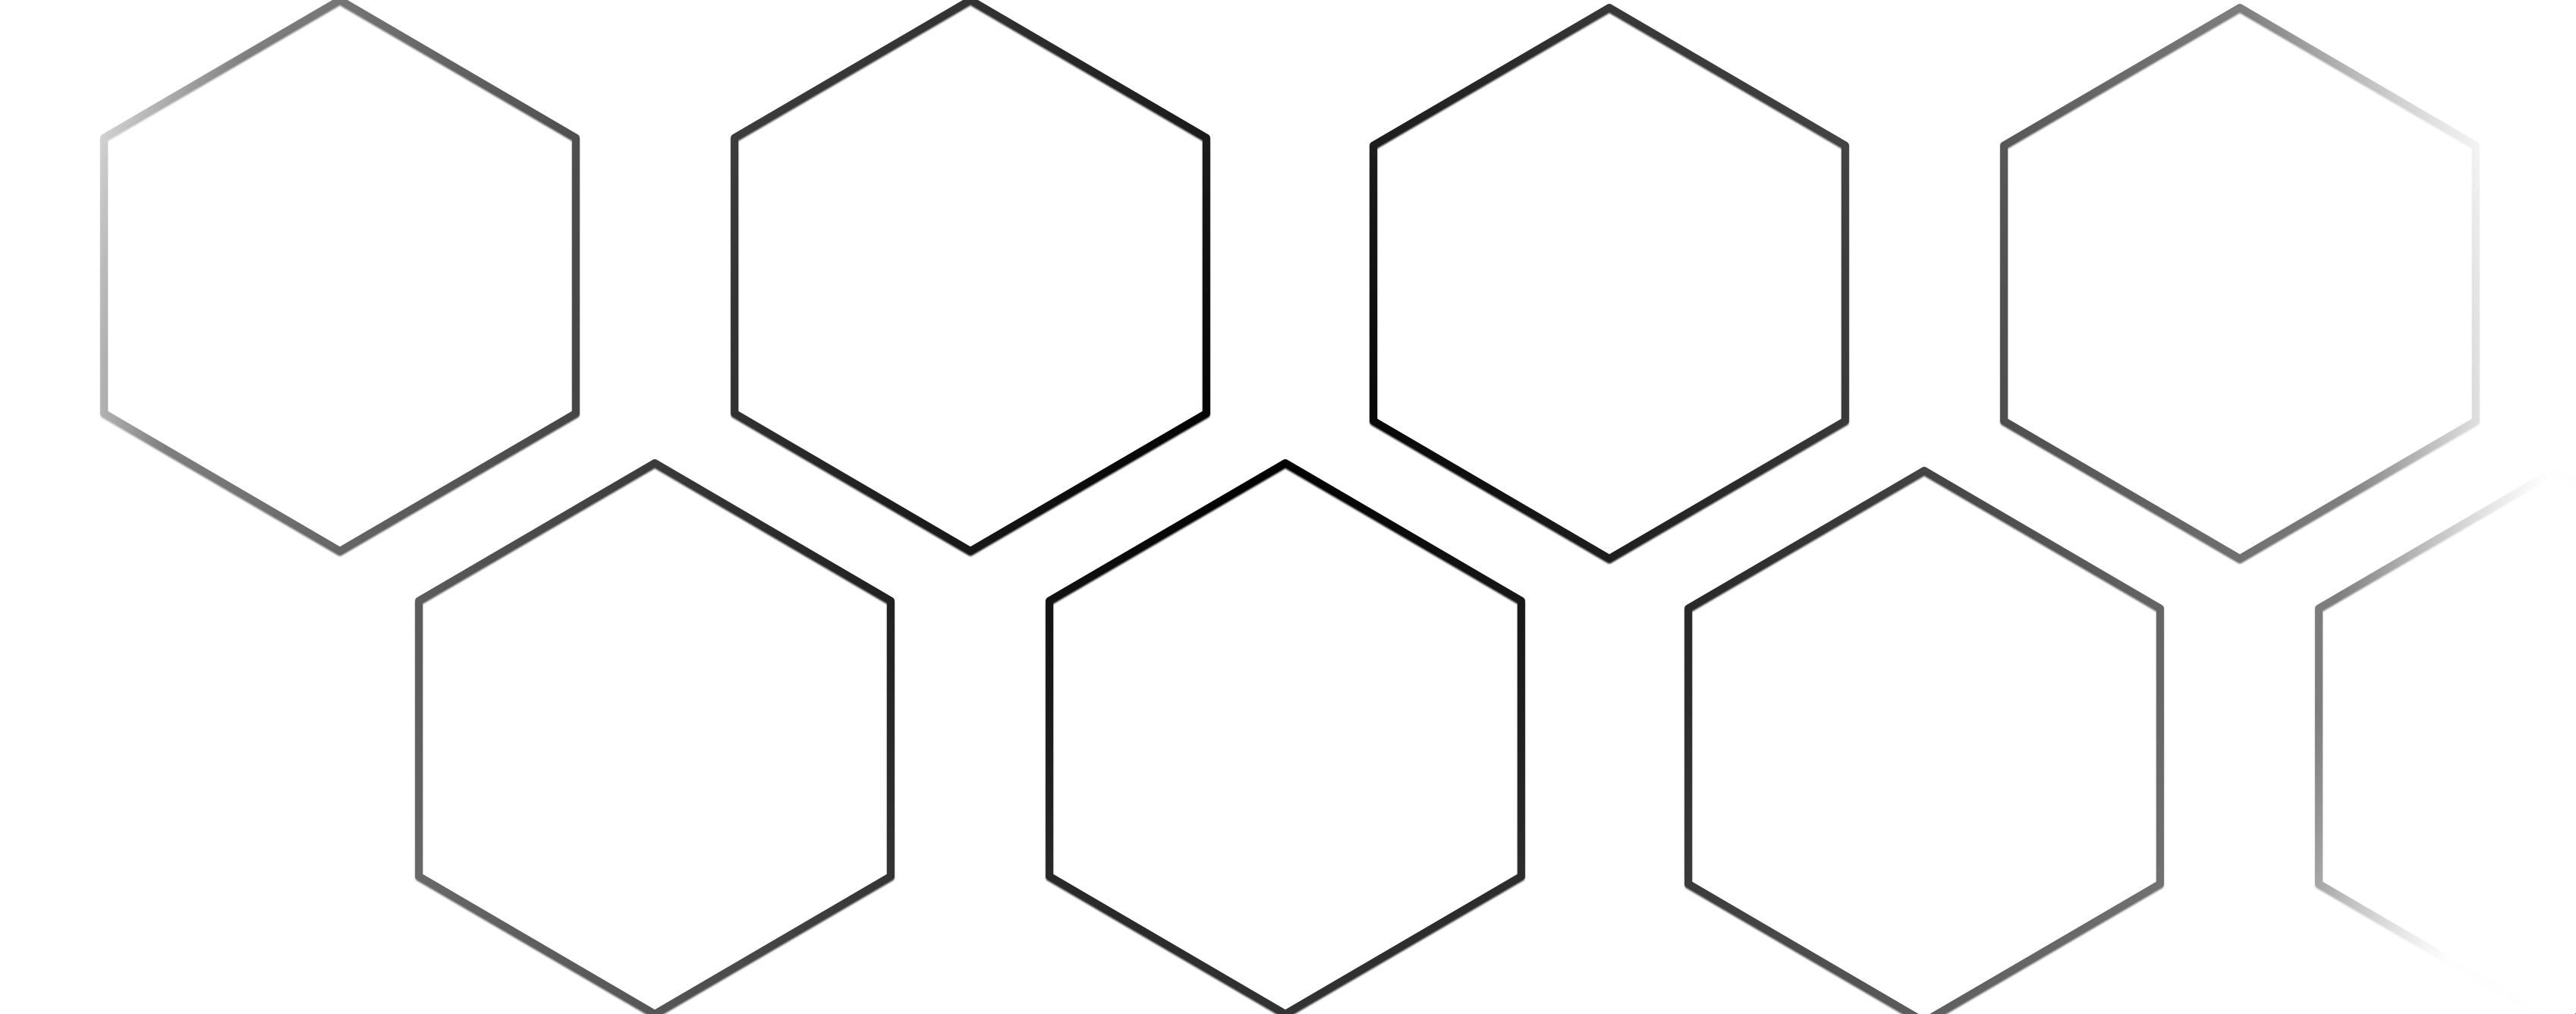
\includegraphics[width=\textwidth]{figures/complexity/hexblend.png}
      \vspace{5mm}
      \includegraphics<3->[width=\textwidth]{figures/complexity/decompose.png}
    \end{overlayarea}
  \end{figure}
\end{column}

\begin{column}[T]{0.25\textwidth}
\centering
\vspace{8mm}

\only<1>{
  \vspace{6.8mm}
}

\only<2->{
\small{Complexity}
\vspace{3mm}
}

\vspace{7mm}



% \only<2->{
\small{Tasks}
% }

\vspace{10mm}

\only<3->{\small{Decomposition}}

\end{column}
\end{columns}
\end{frame}

\end{document}